\documentclass[11pt]{article}

\usepackage[a4paper,margin=1in]{geometry}
\usepackage[T1]{fontenc}
\usepackage[utf8]{inputenc}
\usepackage{lmodern}
\usepackage{graphicx}
\usepackage{subcaption}
\usepackage{booktabs}
\usepackage{hyperref}
\usepackage{float}
\usepackage{tabularx}
\usepackage{longtable}
\usepackage{array}
\usepackage{makecell}
\usepackage{ragged2e}
\usepackage{adjustbox}
\usepackage{xurl}
\usepackage{seqsplit}
\usepackage{microtype}
\usepackage{amsmath}

\newcolumntype{L}[1]{>{\RaggedRight\arraybackslash}p{#1}}
\newcolumntype{Y}{>{\RaggedRight\arraybackslash}X}
\newcommand{\code}[1]{\path{#1}}
\newcommand{\pathcode}[1]{\path{#1}}
\setcounter{table}{0}
\renewcommand{\thetable}{S\arabic{table}}
\setcounter{figure}{0}
\renewcommand{\thefigure}{S\arabic{figure}}

\title{Supplementary Material: City1 Unified Framework}
\author{}
\date{}

\begin{document}

\maketitle

\section*{Supplement Overview}

This supplement retains the expanded evidence logic and technical appendices for the unified City1 framework paper. It preserves the deterministic baseline evidence matrix, the uncertainty-aware evidence matrix, a combined evidence matrix, the city registry, the frozen feature inventory, weak-target weights, calibration and confidence rules, hotspot class definitions, detailed qualitative cases, example surface maps, file manifests, and explicit limitation notes.


\section{S1. Deterministic Validation-Evidence Matrix}

Supplementary Table~S1 reproduces the full deterministic validation-evidence matrix and its claim boundaries.

\begingroup
\small
\setlength{\LTleft}{0pt}
\setlength{\LTright}{0pt}
\begin{longtable}{L{0.14\textwidth} L{0.18\textwidth} L{0.16\textwidth} L{0.20\textwidth} L{0.22\textwidth}}
\caption{Deterministic validation-evidence matrix for the unified City1 framework.}\label{tab:s1-deterministic-evidence}\\
\toprule
Validation layer & Question answered & Metric / artifact used & What it supports & What it does not support \\
\midrule
\endfirsthead
\toprule
Validation layer & Question answered & Metric / artifact used & What it supports & What it does not support \\
\midrule
\endhead
\bottomrule
\endfoot
LOCO & Does the baseline transfer to unseen cities? & Calibrated RMSE and calibrated $R^2$ across hold-out cities & Cross-city transferability under data scarcity & Within-city local correctness or cell-level truth \\
Spatial block CV & Does performance remain stable when local leakage is restricted? & Blocked within-city cross-validation metrics & Within-city robustness under stricter spatial separation & Transfer to unseen cities or truth validation \\
Grid benchmark & Which operating resolution best balances detail and stability? & Benchmark score across 250 m, 500 m, and 1000 m grids & Fixed production choice for the main operating grid & A universal claim that one grid size is optimal in every setting \\
OSM completeness & How much open-data support is available by city? & Completeness score, label, and zero-share diagnostics & Interpretation confidence and caution context & Predictive accuracy or validation against population truth \\
District benchmark & Does the surface remain coherent after aggregation to available districts? & District-level Pearson and Spearman correlations & Partial internal administrative coherence where references exist & Cell-level truth validation or uniform reliability across cities \\
External benchmark & Do independent products agree with broad structure or hotspots? & Pearson, Spearman, top-decile overlap, hotspot IoU & External structural plausibility from independent products & Ground-truth validation or proof that an external product is correct \\
Ablation & Which feature families carry the dominant predictive structure? & LOCO RMSE and $R^2$ by ablation family & Role of built form, broader features, and calibration & Feature-level causality or a full explainability layer \\
Qualitative plausibility & Do curated hotspot and coldspot cases look urban-structurally plausible? & Overview maps and detailed curated case panels & Map plausibility and urban-structural interpretation & Quantitative validation or census-equivalent truth claims \\
\end{longtable}
\endgroup




\section{S2. Uncertainty Validation-Evidence Matrix}

Supplementary Table~S2 records the evidence logic for the uncertainty-aware stage and its claim boundaries.

\begin{longtable}{L{2.7cm}L{3.2cm}L{4.3cm}L{4.3cm}}
\caption{Uncertainty validation-evidence matrix for the unified City1 framework.}\label{tab:s2-uncertainty-evidence}\\
\toprule
Evidence layer & Main artifact & What it supports & What it does not support \\
\midrule
\endfirsthead
\toprule
Evidence layer & Main artifact & What it supports & What it does not support \\
\midrule
\endhead
Interval coverage against proxy targets & Table 9, Figure 9 & Bounded interval behavior against weak/proxy targets under LOCO-like and inference-only checks & True census coverage or full probabilistic calibration \\
Error-vs-uncertainty alignment & Table 10, Figure 9 & Positive association between proxy-target error and uncertainty width & Uniform ranking between confidence score and true error, or truth-level calibration \\
District aggregation evidence & Table 13 & Partial administrative support after aggregation for Almaty, Astana, and Shymkent & Full district interval coverage or cell-level administrative truth \\
External disagreement alignment & Table 13 & Structural comparison context against WorldPop and GHS-POP & External products as ground truth or a strong claim that disagreement always rises with uncertainty \\
Hotspot stability & Table 12, Figure 10 & Separation between stable screening classes and caution-heavy classes & Definitive verification of hotspot correctness \\
Confidence-band validation & Table 11, Figure 7 & Separation of uncertainty burden across high, medium, and low interpretation bands & Probability of correctness or direct truth probability \\
\bottomrule
\end{longtable}




\section{S3. Combined Framework Evidence Matrix}

Supplementary Table~S3 merges both stages into one evidence matrix with an explicit stage-supported column.

\begingroup
\scriptsize
\setlength{\LTleft}{0pt}
\setlength{\LTright}{0pt}
\begin{longtable}{L{0.15\textwidth}L{0.15\textwidth}L{0.18\textwidth}L{0.18\textwidth}L{0.18\textwidth}L{0.10\textwidth}}
\caption{Combined evidence matrix for the unified City1 framework.}\label{tab:s3-combined-evidence}\\
\toprule
Evidence layer & Main artifact & Question answered & What it supports & What it does not support & Stage supported \\
\midrule
\endfirsthead
\toprule
Evidence layer & Main artifact & Question answered & What it supports & What it does not support & Stage supported \\
\midrule
\endhead
LOCO & Table 3 & Does the calibrated baseline transfer to unseen cities? & Cross-city transferability under data scarcity & Cell-level truth validation & baseline \\
Spatial block CV & Table 3 & Does within-city performance remain stable under stricter separation? & Within-city robustness & Unseen-city truth validation & baseline \\
Grid benchmark & Table 3, Figure 2 & Which grid best balances detail and stability? & Fixed production choice at 500 m & A universal optimal-grid claim & baseline \\
OSM completeness & Figure 3, Table 2 & How strong is open-data support by city? & Interpretation context & Predictive accuracy proof & baseline \\
District benchmark & Table 4, Figure 3 & Does the baseline remain coherent after aggregation? & Partial administrative support & Cell-level truth & baseline \\
External benchmark & Table 5, Figure 4 & Do independent gridded products align structurally? & Structural plausibility & Ground truth & baseline \\
Ablation & Table 6 & Which feature families dominate the baseline? & Dominant predictive structure and value of calibration & Feature-level causality & baseline \\
Qualitative plausibility & Figure 5, Supplement S7 & Do curated cases remain urban-structurally plausible? & Plausibility and interpretability & Quantitative truth validation & baseline \\
Interval coverage & Table 9, Figure 9 & Do proxy intervals contain retained proxy targets? & Bounded interval behavior & True census coverage & uncertainty \\
Error-width alignment & Table 10, Figure 9 & Does higher uncertainty width align with higher proxy-target error? & Useful error signal in width & Full probabilistic calibration & uncertainty \\
Confidence-band validation & Table 11, Figure 7 & Do bands separate uncertainty burden? & Interpretation support differentiation & Probability of correctness & uncertainty \\
Hotspot stability & Table 12, Figure 10 & Are stable classes more stable than caution-heavy classes? & Screening reliability & Verified hotspot truth & uncertainty \\
District interval evidence & Table 13 & Is district interval support fully available? & Partial after-aggregation support only & Solved district interval validation & uncertainty \\
External disagreement alignment & Table 13 & Does uncertainty rise systematically with external disagreement? & Structural comparison context & Strong monotonicity claim or truth proof & uncertainty \\
\bottomrule
\end{longtable}
\endgroup




\section{S4. City Registry, Coverage, and Feature Inventory}

Supplementary Table~S4 gives the full city registry and coverage roles retained in the deterministic package. Supplementary Table~S5 lists the frozen feature inventory by family and shows which features participate directly in the weak-target construction.

\begingroup
\small
\setlength{\LTleft}{0pt}
\setlength{\LTright}{0pt}
\begin{longtable}{L{0.14\textwidth} L{0.20\textwidth} L{0.20\textwidth} L{0.12\textwidth} L{0.12\textwidth} L{0.12\textwidth}}
\caption{City registry and coverage roles in the unified City1 framework. Completeness context is shown only where feature generation was available in the reference package.}\label{tab:s4-city-registry}\\
\toprule
City & Framework role & Official totals provenance & District benchmark & Qualitative anchor & Completeness context \\
\midrule
\endfirsthead
\toprule
City & Framework role & Official totals provenance & District benchmark & Qualitative anchor & Completeness context \\
\midrule
\endhead
\bottomrule
\endfoot
Almaty & validated baseline city; reliability-evidence city & manual verified BNS record & yes & yes & good \\
Astana & validated baseline city; reliability-evidence city & manual verified BNS record & yes & yes & moderate \\
Shymkent & validated baseline city; reliability-evidence city & manual verified BNS record & yes & no & moderate \\
Semey & validated baseline city; smoke-passed example; reliability-evidence city & workbook-derived BNS record & no & no & good \\
Taraz & validated baseline city & workbook-derived BNS record & no & no & good \\
Uralsk & validated baseline city & workbook-derived BNS record & no & no & good \\
Petropavlovsk & validated baseline city & workbook-derived BNS record & no & no & good \\
Ust Kamenogorsk & validated baseline city & workbook-derived BNS record & no & no & good \\
Kurchatov & runtime-only calibrated example & workbook-derived BNS record & no & no & n/a \\
Ridder & official-total registry only & workbook-derived BNS record & no & no & n/a \\
\end{longtable}
\endgroup



\begingroup
\small
\renewcommand{\arraystretch}{1.08}
\setlength{\LTleft}{0pt}
\setlength{\LTright}{0pt}
\begin{longtable}{L{0.15\textwidth} L{0.24\textwidth} L{0.10\textwidth} L{0.37\textwidth}}
\caption{Frozen feature inventory grouped by family. The weak-target column indicates whether a feature participates directly in the default weak-label weighting scheme.}\label{tab:s5-feature-inventory}\\
\toprule
Family & Feature & Weak target & Frozen role \\
\midrule
\endfirsthead
\toprule
Family & Feature & Weak target & Frozen role \\
\midrule
\endhead
\bottomrule
\endfoot
Built form & Building\_Count & yes & count of intersecting building footprints within the grid cell \\
Built form & Building\_Area & yes & total intersecting building footprint area \\
Built form & Residential\_Area & yes & intersecting area of residential building types \\
Built form & Commercial\_Area & no & intersecting area of commercial or office building types \\
Built form & Retail\_Area & no & intersecting area of retail-oriented building types \\
Built form & Public\_Area & no & intersecting area of public-service building types \\
Built form & \shortstack[l]{Building\_With\\Levels\_Count} & no & number of buildings with observed level tags \\
Built form & Mean\_Building\_Levels & no & mean observed building levels where level tags are present \\
Floor area & Total\_Floor\_Area & yes & area weighted by observed or fallback building levels \\
Transport & Road\_Length & yes & total intersecting road length in the grid cell \\
Transport & Bus\_Stop\_Count & yes & count of intersecting bus-stop points \\
POI/services & Park\_Area & no & total intersecting park area \\
POI/services & Schools\_Count & yes & count of intersecting school or kindergarten points \\
POI/services & Hospitals\_Count & yes & count of intersecting hospital or clinic points \\
POI/services & Parks\_Shops\_Count & yes & combined count of parks and shop features used in the fixed stack \\
POI/services & POI\_Access\_Index & no & inverse-distance access proxy to nearby OSM activity points \\
Composite & Combined\_Index & yes & normalized aggregate index spanning major built-form, transport, park, and floor-area signals \\
\end{longtable}
\endgroup



\section{S5. Weak Target, Calibration, and Confidence Rules}

The weak-target construction used by the deterministic stage is:
\[
s_i = \sum_{k \in K} w_k \cdot \mathrm{MinMax}\!\left(\log\!\left(1 + \max(x_{ik}, 0)\right)\right),
\]
\[
\tilde{s}_i = s_i + \epsilon,
\qquad
q_i = \frac{\tilde{s}_i}{\sum_{j \in c} \tilde{s}_j},
\qquad
y_i^{\mathrm{weak}} = q_i \cdot P_c.
\]
Here $P_c$ is the official total for city $c$, so the weak target is an officially anchored proxy allocation rather than a ground-truth cell label.

The deterministic calibration rule is:
\[
\hat{y}_i^{\mathrm{cal}} = \hat{y}_i \cdot \frac{P_c}{\sum_{j \in c} \hat{y}_j}.
\]
If the within-city prediction sum is non-positive, the workflow falls back to uniform allocation.

The uncertainty-aware confidence formula is:
\[
\mathrm{confidence}_i =
\operatorname{clip}\!\left(
0.40\,s_i +
0.25\,o_c +
0.20\,e_i +
0.15\,d_c, 0, 1
\right),
\]
where
\[
s_i = 1 - \operatorname{clip}\!\left(
\frac{r_i}{\max(q_{0.90}^{(c)},\epsilon)}, 0, 1
\right),
\qquad
r_i = \frac{\mathrm{P90}_i - \mathrm{P10}_i}{\max(\mathrm{P50}_i,\epsilon)}.
\]

Supplementary Table~S6 records the weak-target weights, and Table~S7 records the hotspot class definitions used for screening.

\begin{table}[H]
\centering
\small
\caption{Weak-label weights used in the fixed proxy score. Only features available in a given city contribute to the weighted sum.}
\label{tab:s6-weak-label-weights}
\begin{tabular}{lll}
\toprule
Feature & Weight & Family \\
\midrule
Total\_Floor\_Area & 0.35 & floor area \\
Building\_Area & 0.18 & built form \\
Residential\_Area & 0.16 & built form \\
Building\_Count & 0.08 & built form \\
Road\_Length & 0.06 & transport \\
Bus\_Stop\_Count & 0.04 & transport \\
Schools\_Count & 0.03 & POI/services \\
Hospitals\_Count & 0.03 & POI/services \\
Parks\_Shops\_Count & 0.04 & POI/services \\
Combined\_Index & 0.03 & composite \\
\bottomrule
\end{tabular}
\end{table}



\begin{table}[H]
\centering
\footnotesize
\setlength{\tabcolsep}{3.5pt}
\renewcommand{\arraystretch}{1.15}
\caption{Hotspot-class definitions used in the uncertainty-aware stage. Short display labels are shown in the table; exact code identifiers are listed below.}
\label{tab:s7-hotspot-class-definitions}
\begin{tabularx}{\textwidth}{L{3.25cm} Y Y}
\toprule
Display class & Operational definition & Interpretation rule \\
\midrule
High-value / high-confidence & Top decile by calibrated P50 within city and confidence band = high & Strongest screening candidate; not verified census truth \\
High-value / low-confidence & Top decile by calibrated P50 within city and confidence band = low & Potentially important hotspot that remains review-oriented \\
Medium-value / high-confidence & P50 between city P75 and P90 with confidence band = high & Secondary stable screening candidate \\
Low-value / high-uncertainty & Below city median P50 with confidence band = low & Caution-heavy class; not a firm planning target \\
Not priority & All remaining cells & Background class outside the prioritization focus \\
\bottomrule
\end{tabularx}
\par\medskip
\noindent\footnotesize Exact identifiers:
\begin{itemize}\setlength{\itemsep}{0pt}\setlength{\topsep}{0pt}
\item \code{high_value_high_confidence}
\item \code{high_value_low_confidence}
\item \code{medium_value_high_confidence}
\item \code{low_value_high_uncertainty}
\item \code{not_priority}
\end{itemize}
\end{table}



\section{S6. Hotspot Classes and Limitation Tables}

Supplementary Table~S8 consolidates the major limitation rules that must remain visible in the unified manuscript.

\begin{longtable}{L{3.2cm}L{4.0cm}L{5.6cm}}
\caption{Framework-level limitations that must remain explicit in the unified manuscript.}\label{tab:s8-framework-limitations}\\
\toprule
Limitation & Affected evidence & Manuscript rule \\
\midrule
\endfirsthead
\toprule
Limitation & Affected evidence & Manuscript rule \\
\midrule
\endhead
Missing cell-level truth & Entire framework & Never describe outputs as observed cell-level census counts \\
Weak/proxy target validation & Deterministic and uncertainty tables & Describe model scores and interval behavior as proxy-target evidence \\
OSM quality variation & Deterministic and uncertainty city interpretation & Use completeness as interpretation context, not as accuracy proof \\
Partial district support & Deterministic Table 4 and uncertainty Table 13 & Preserve that district evidence is partial after aggregation \\
External products are not truth & External comparison in both stages & Use structural-comparison wording only \\
\texttt{confidence\_score} is not probability & Framework and uncertainty stage & Use ``interpretation confidence'' wording only \\
Bounded LOCO-like configuration & Uncertainty Table 9 and Table 10 & State that held-out local evidence used 5 members and 60 trees \\
No true census uncertainty & Entire uncertainty stage & Never describe intervals as true census-uncertainty intervals \\
\bottomrule
\end{longtable}




\section{S7. Detailed Qualitative Cases and Example Surfaces}

The detailed qualitative hotspot and coldspot cases are retained here because they support the main-paper plausibility narrative without overloading the core text.

\begin{figure}[H]
\centering
\begin{subfigure}[t]{0.48\textwidth}
    \centering
    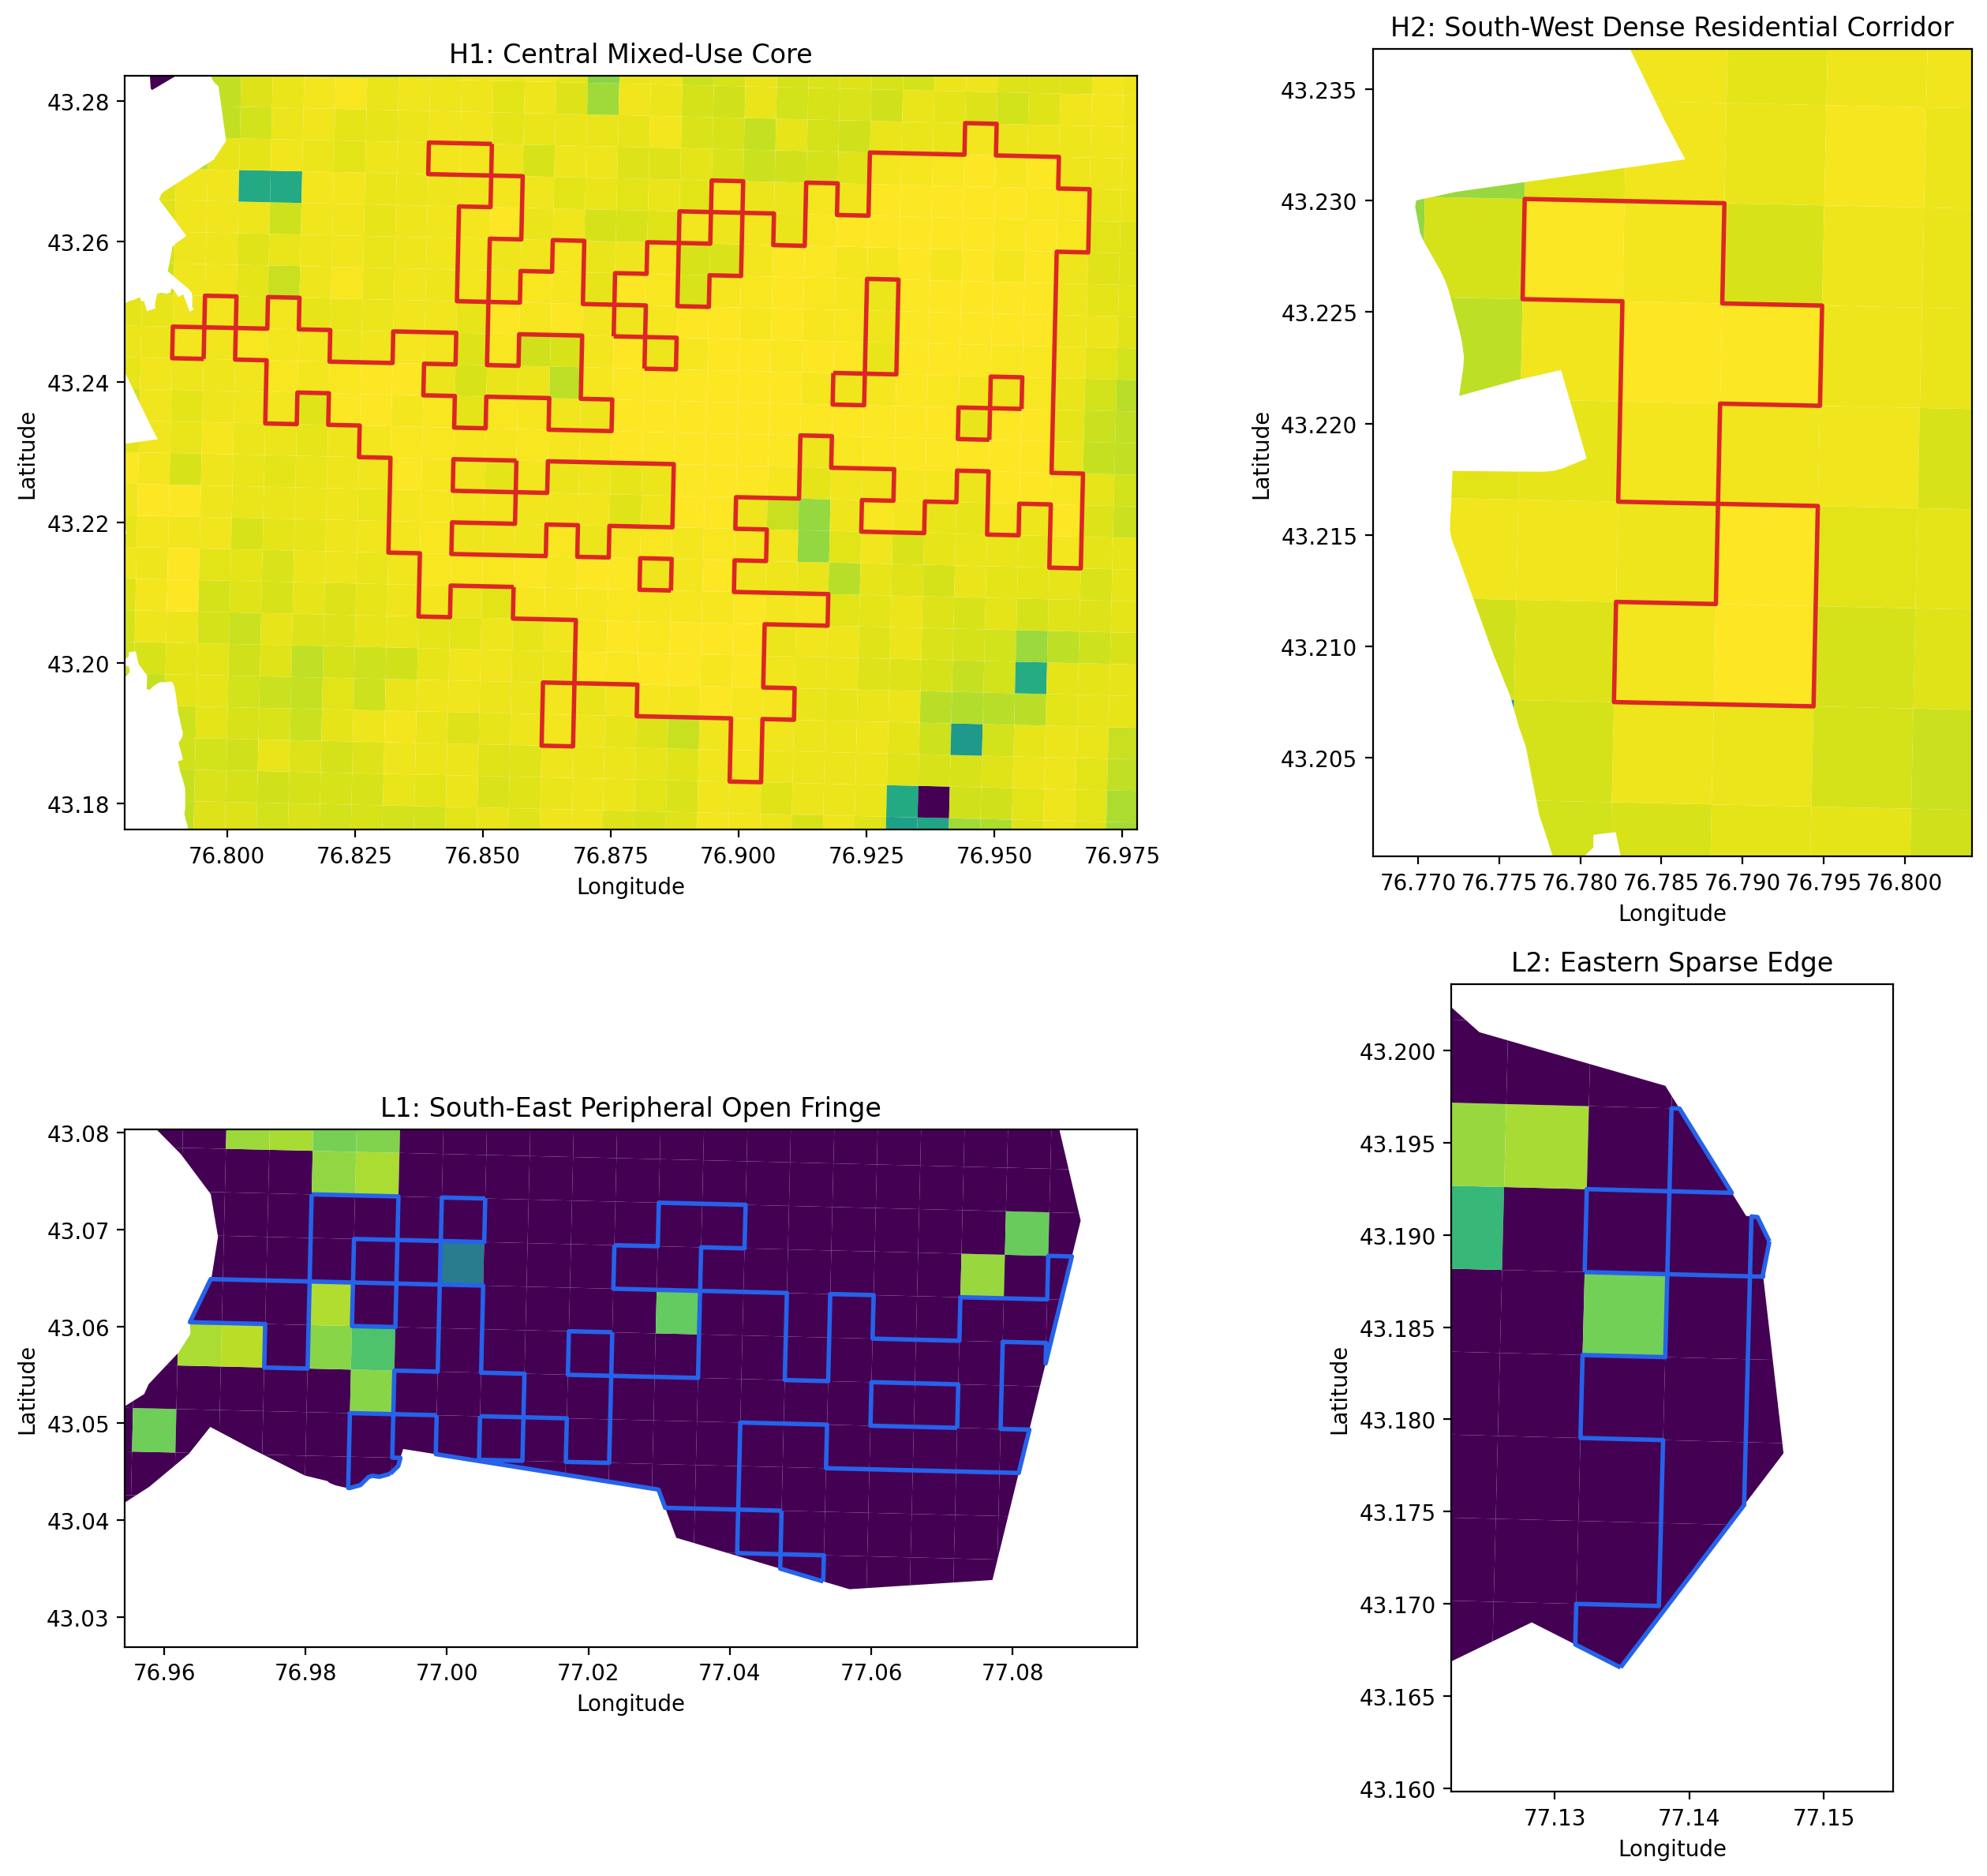
\includegraphics[width=\textwidth]{figures/figure_qualitative_cases_almaty.png}
    \caption{Almaty detailed cases}
\end{subfigure}
\hfill
\begin{subfigure}[t]{0.48\textwidth}
    \centering
    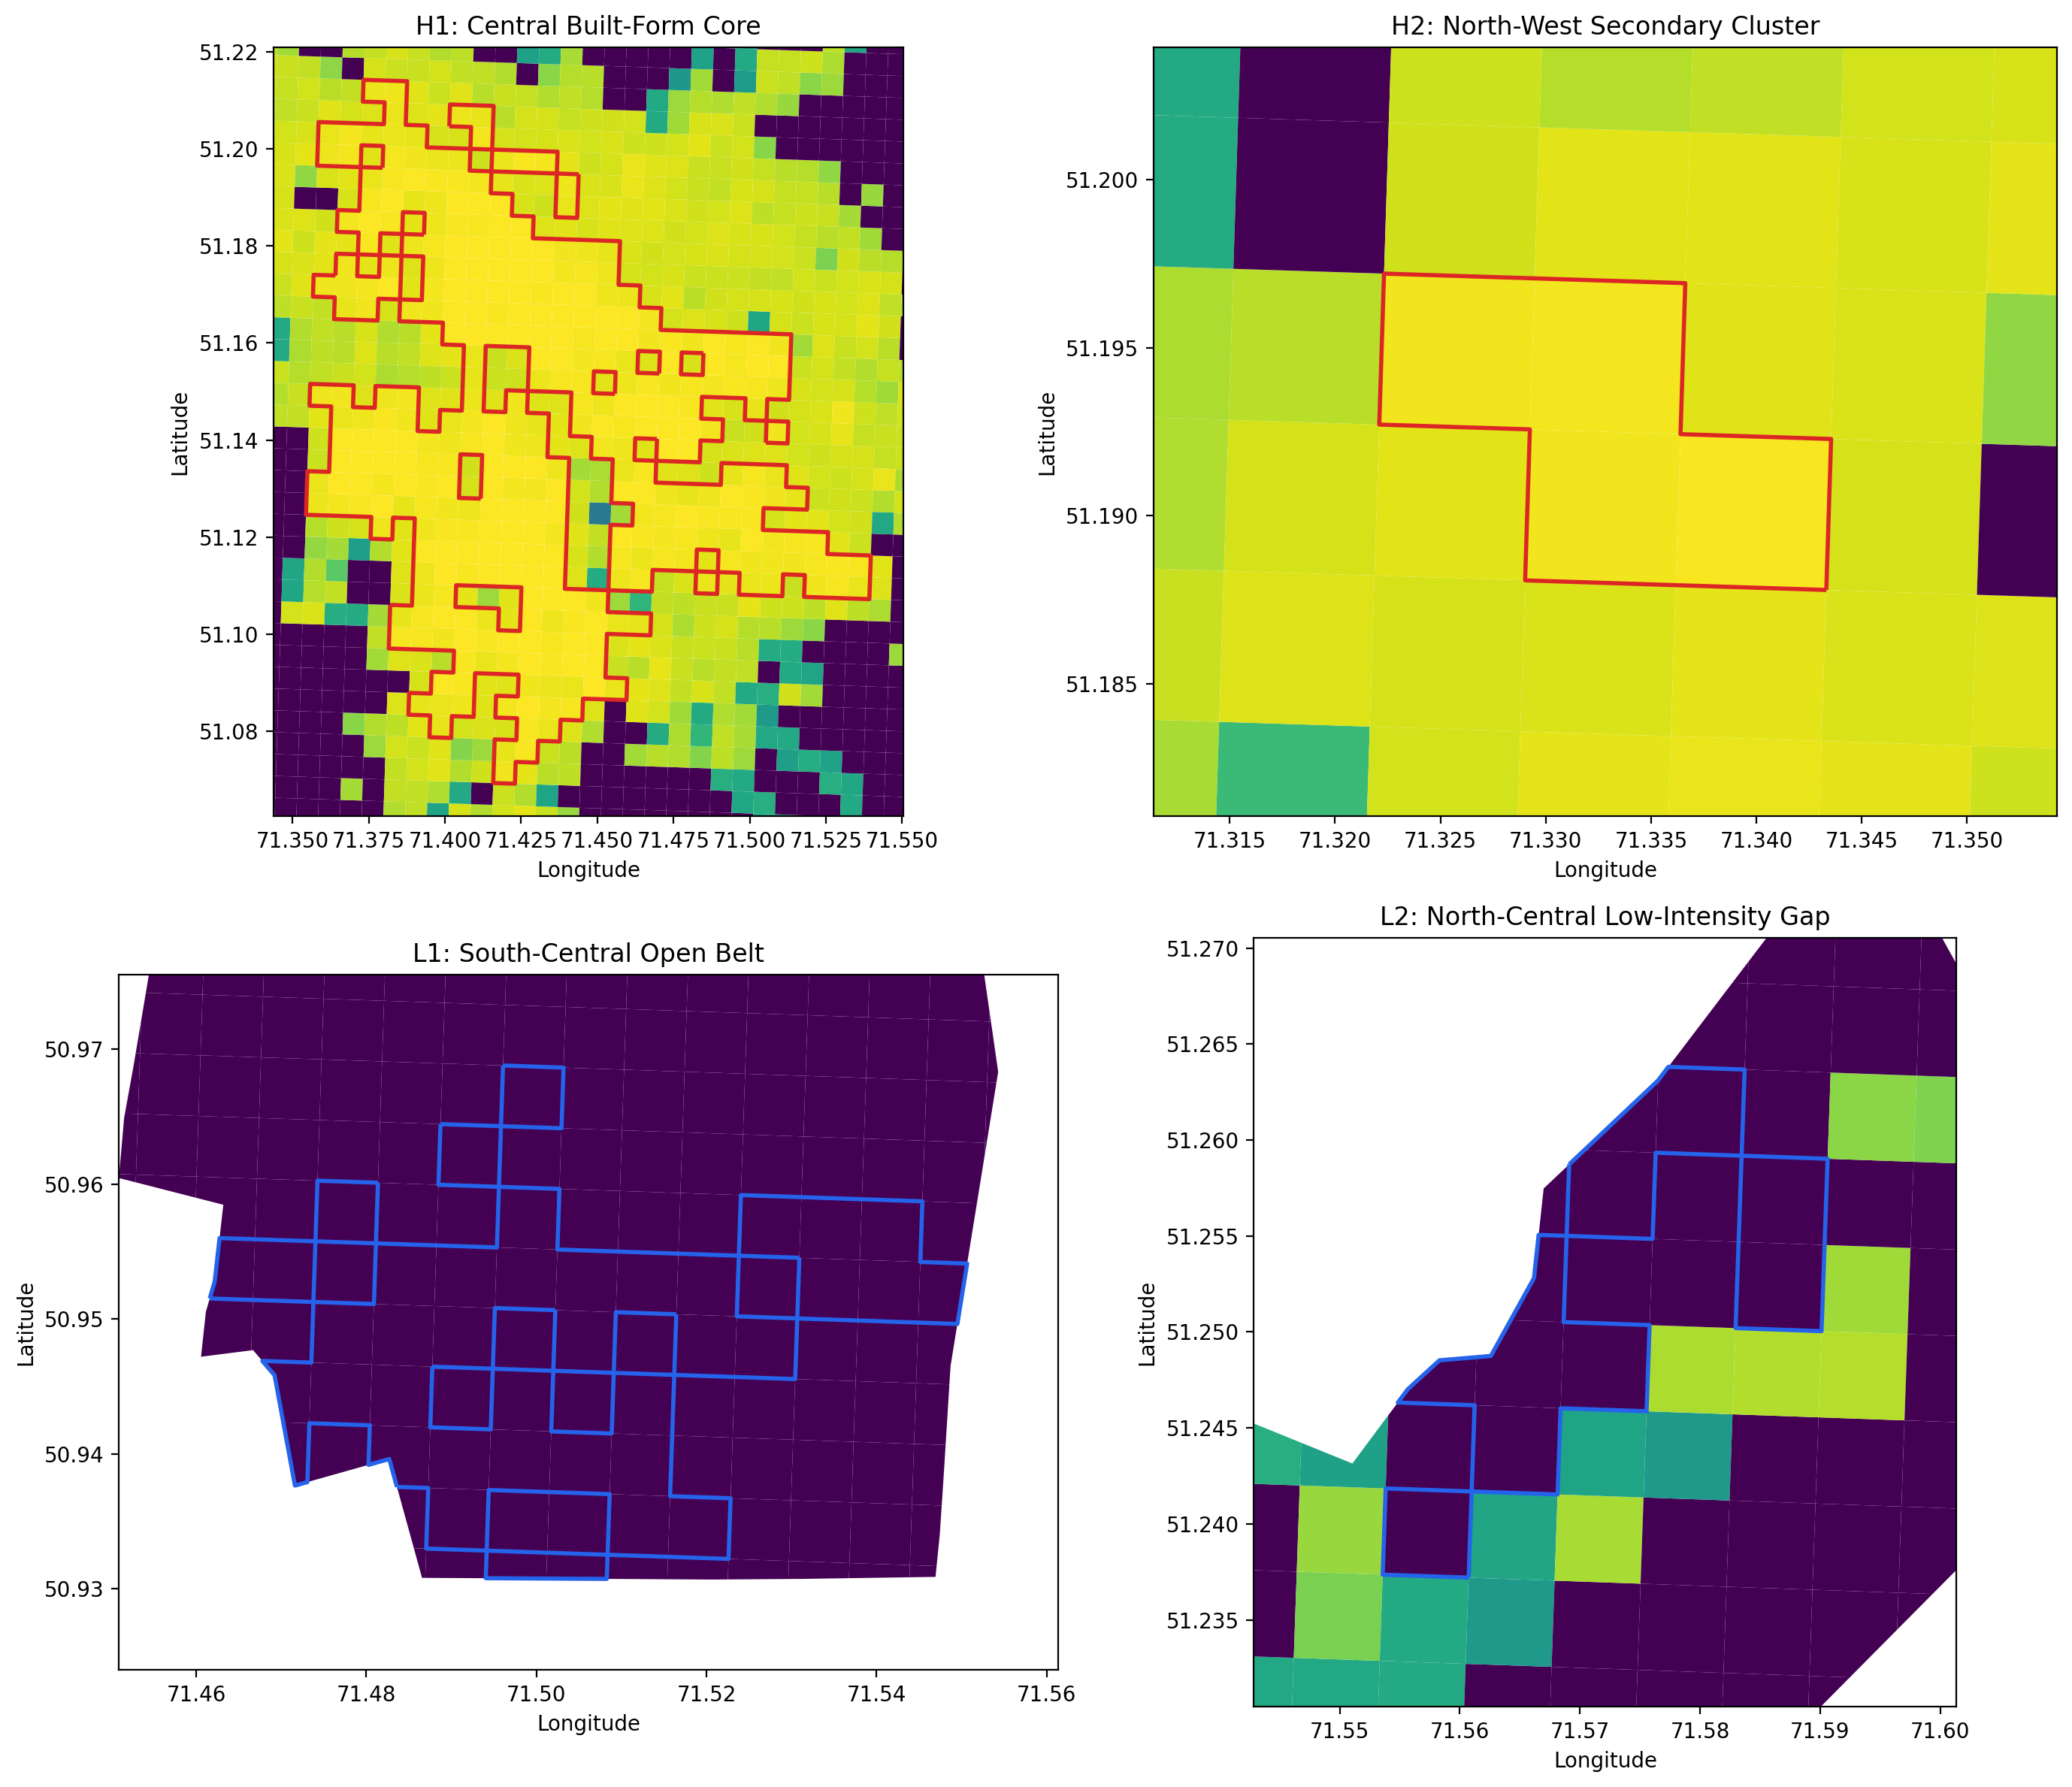
\includegraphics[width=\textwidth]{figures/figure_qualitative_cases_astana.png}
    \caption{Astana detailed cases}
\end{subfigure}
\caption{Detailed qualitative cases for the deterministic stage. These panels support plausibility reading rather than truth validation.}
\end{figure}

\begin{figure}[H]
\centering
\begin{subfigure}[t]{0.48\textwidth}
    \centering
    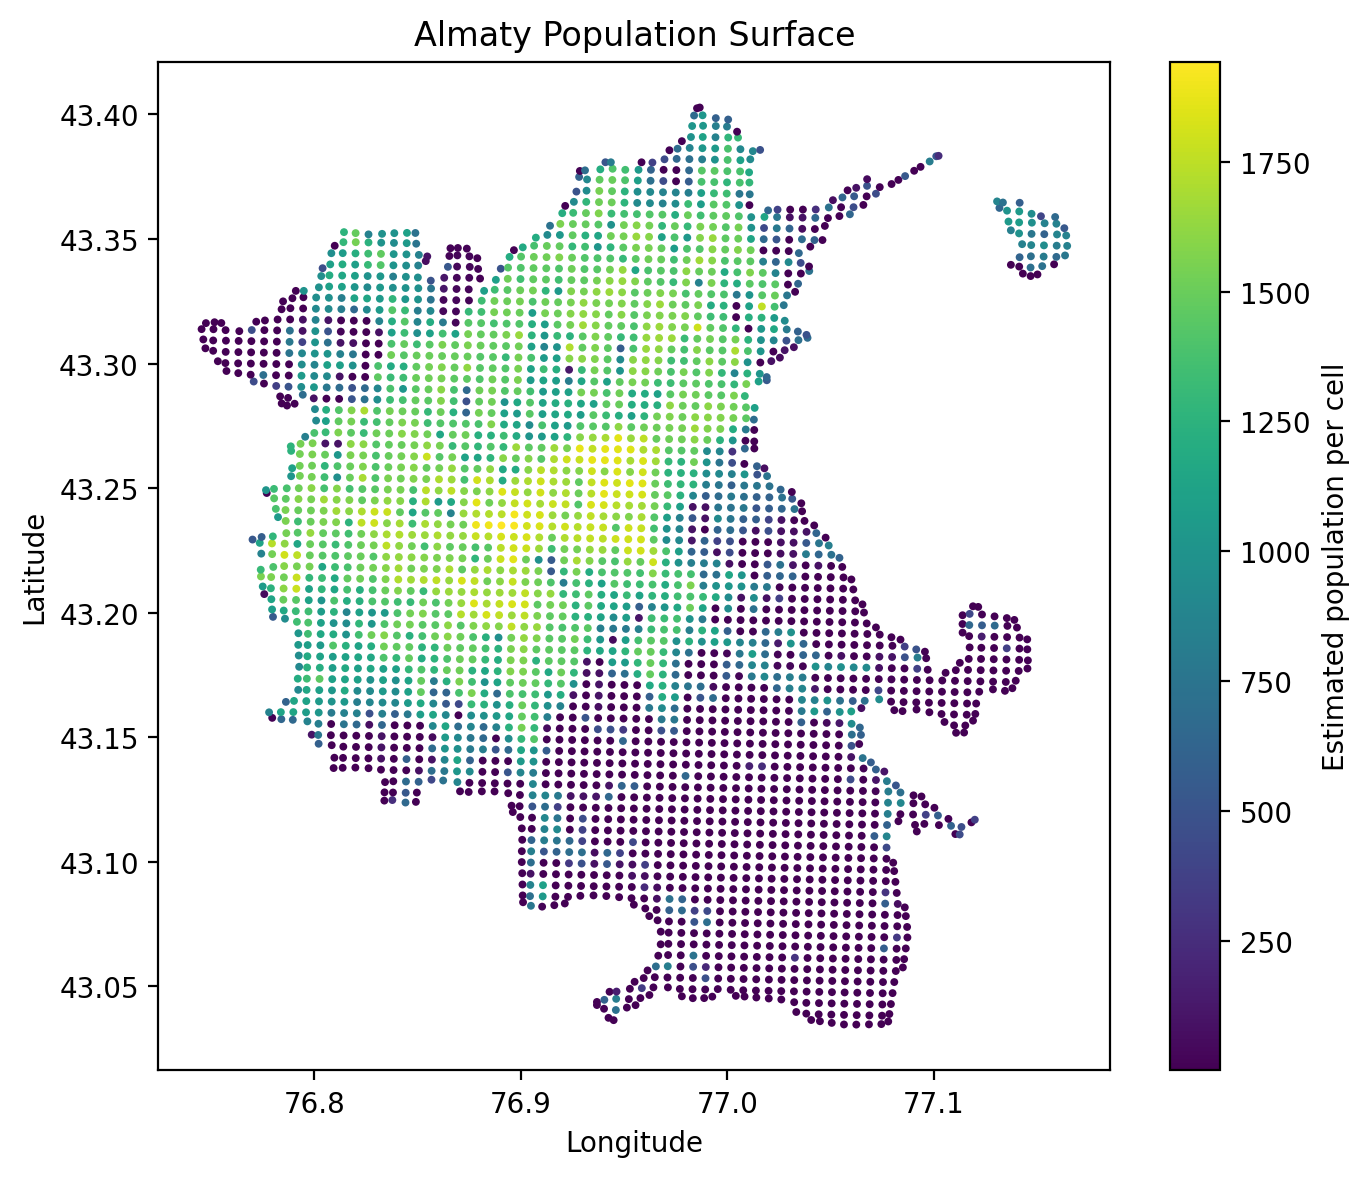
\includegraphics[width=\textwidth]{figures/figure_surface_almaty.png}
    \caption{Almaty example surface}
\end{subfigure}
\hfill
\begin{subfigure}[t]{0.48\textwidth}
    \centering
    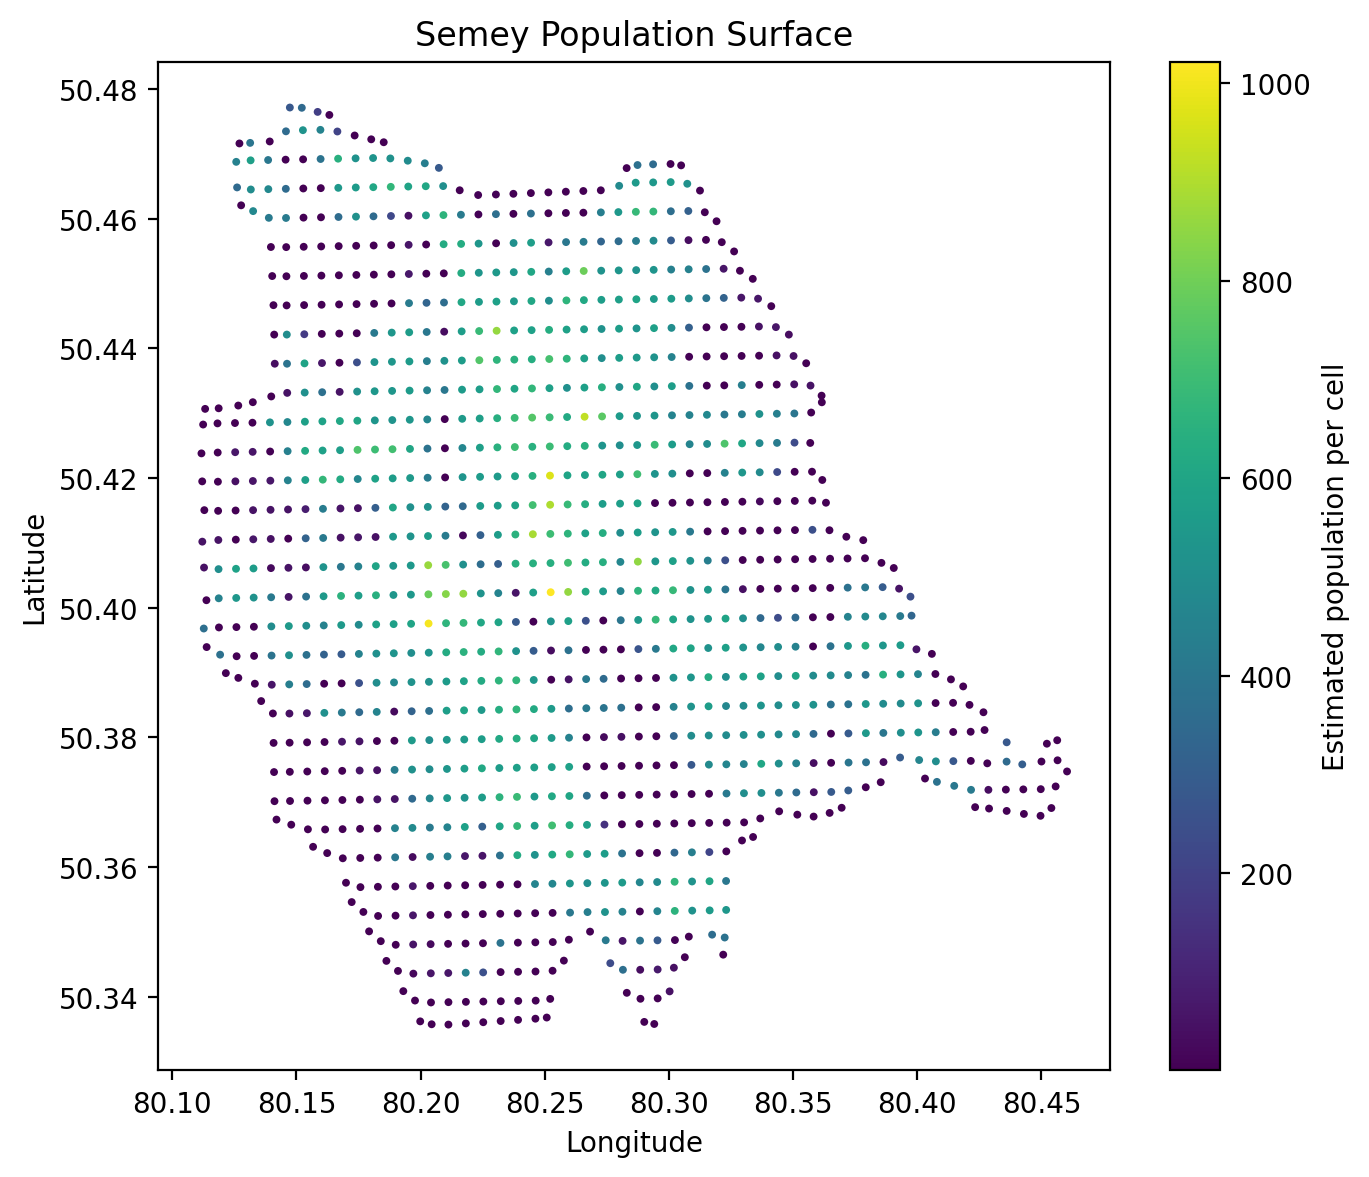
\includegraphics[width=\textwidth]{figures/figure_surface_semey.png}
    \caption{Semey example surface}
\end{subfigure}
\caption{Additional example proxy population surfaces retained for supplementary inspection.}
\end{figure}

\begin{figure}[H]
\centering
\begin{subfigure}[t]{0.48\textwidth}
    \centering
    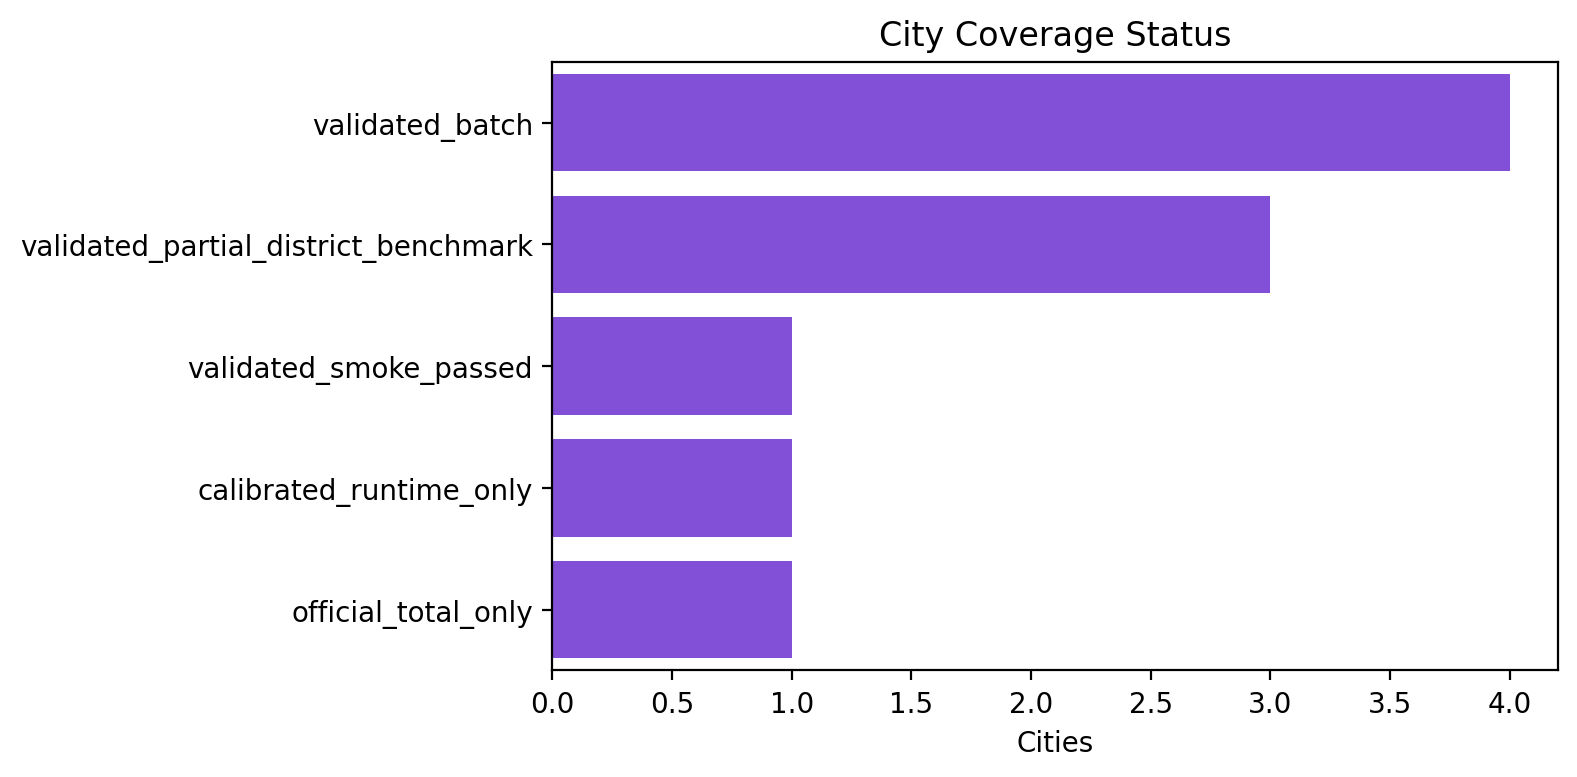
\includegraphics[width=\textwidth]{figures/figure_city_status.png}
    \caption{City status overview}
\end{subfigure}
\hfill
\begin{subfigure}[t]{0.48\textwidth}
    \centering
    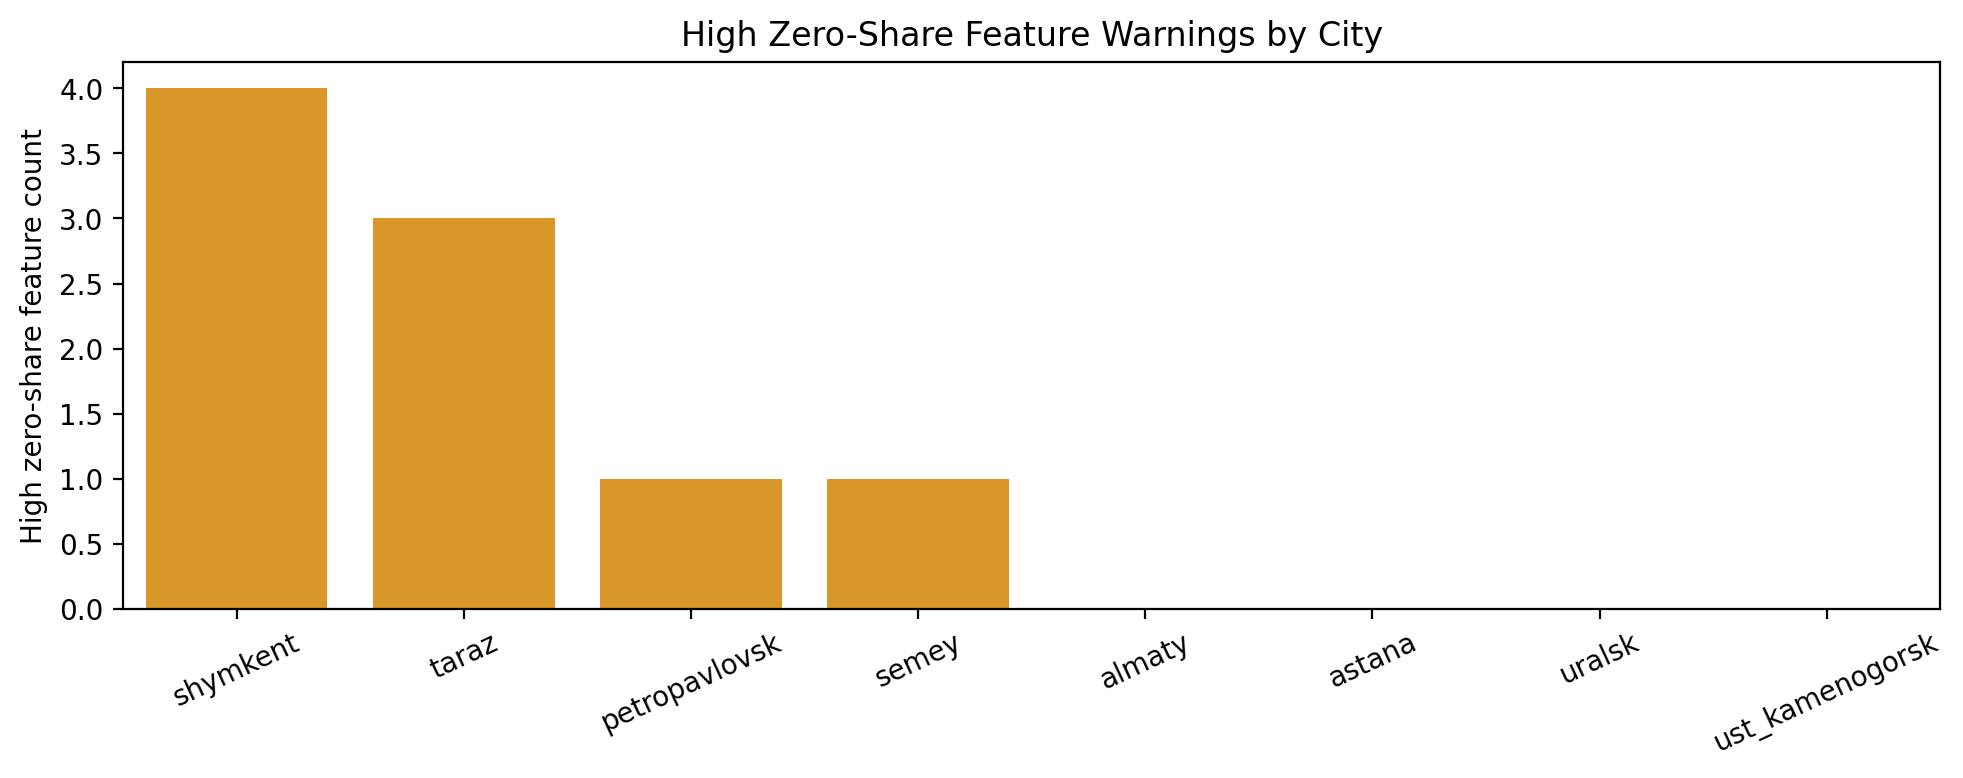
\includegraphics[width=\textwidth]{figures/figure_qa_warnings.png}
    \caption{QA warnings overview}
\end{subfigure}
\caption{Supplementary reference figures from the deterministic package that document registry status and QA context.}
\end{figure}


\section{S8. File Manifests and Supporting Material}

Supplementary Table~S9 lists the key fixed source files used to assemble the unified framework paper.

\begin{table}[H]
\centering
\footnotesize
\setlength{\tabcolsep}{4pt}
\renewcommand{\arraystretch}{1.15}
\caption{Compact artifact manifest for the main fixed source materials used in the unified framework paper.}
\label{tab:s9-file-manifest}
\begin{tabularx}{\textwidth}{L{3.45cm} L{3.3cm} L{3.0cm} Y}
\toprule
Artifact group & Source artifact & Role & Use in unified manuscript \\
\midrule
Deterministic manuscript package & main manuscript file & deterministic manuscript & Stage 1 narrative backbone \\
Deterministic supplement package & supplement file & deterministic supplement & deterministic appendices and support material \\
Deterministic paper-facing artifacts & tables and figures & deterministic evidence & baseline quantitative and visual anchors \\
Uncertainty manuscript package & main manuscript file & uncertainty manuscript & Stage 2 narrative backbone \\
Uncertainty supplement package & supplement file & uncertainty supplement & uncertainty appendices and support rules \\
Uncertainty paper-facing package & summary and freeze manifest & evidence package & Stage 2 framing, run identity, and limitation boundaries \\
Phase 5 hotspot package & hotspot prioritization report & phase report & hotspot interpretation support \\
Phase 6 validation package & uncertainty validation report & phase report & partial-validation status and limitation wording \\
\bottomrule
\end{tabularx}
\end{table}

\noindent\footnotesize\textit{Representative source paths.}
\begin{itemize}\setlength{\itemsep}{0pt}\setlength{\topsep}{0pt}
\item \pathcode{manuscript_package_v2/main.tex}
\item \pathcode{manuscript_package_v2/supplement.tex}
\item \pathcode{manuscript_package_v2/tables/}
\item \pathcode{manuscript_package_v2/figures/}
\item \pathcode{manuscript_package_v3/main.tex}
\item \pathcode{manuscript_package_v3/supplement.tex}
\item \pathcode{reports/paper_v3_uncertainty/.../paper_summary.md}
\item \pathcode{reports/paper_v3_uncertainty/.../freeze_manifest.json}
\item \pathcode{reports/hotspot_prioritization_v3/.../PHASE_5_HOTSPOT_PRIORITIZATION_REPORT.md}
\item \pathcode{reports/uncertainty_validation_v3/.../PHASE_6_UNCERTAINTY_VALIDATION_REPORT.md}
\end{itemize}
\normalsize


Expanded supporting material retained outside the main narrative includes:

\begin{itemize}
\item deterministic expanded CSV-derived tables:
  \begin{itemize}
  \item \texttt{qa\_city\_summary\_table.csv}
  \item \texttt{grid\_size\_city\_recommendations\_table.csv}
  \item \texttt{external\_benchmark\_metrics\_table.csv}
  \item \texttt{ablation\_selected\_extras\_table.csv}
  \item \texttt{qualitative\_validation\_case\_table.csv}
  \end{itemize}
\item uncertainty phase reports and manifests:
  \begin{itemize}
  \item Phase 5 hotspot prioritization report
  \item Phase 6 uncertainty validation report
  \item Phase 7 paper-facing freeze manifest
  \end{itemize}
\end{itemize}

The main partial-validation notes that must remain visible are:

\begin{itemize}
\item district interval coverage remains partial because frozen district polygon/cell assignment artifacts are unavailable in the light package;
\item the LOCO-like uncertainty evidence used a bounded 5-member, 60-tree configuration;
\item external disagreement alignment is mixed or negative and must not be overstated.
\end{itemize}



\end{document}
